\subsection{Aprendizado por Reforço}

O aprendizado por reforço é uma área de aprendizado de máquina que lida com tomada de decisão sequencial.
Um aspecto chave do aprendizado por reforço é que um agente aprenda uma bom comportamento \cite{franccois2018introduction}.
Isso significa que ele modifica ou adquiri novos comportamentos e habilidades incrementalmente.
Um outro importante aspecto do aprendizado por reforço é que ele usa de experiência de tentativa e erro.
Ademais, o agente do aprendizado por reforço não precisa de completo conhecimento ou controle do ambiente; ele apenas precisa ser capaz de interagir com o ambiente e coletar informações.
Um agente realiza certas ações em um ambiente e um interpretador dá uma recompensa para o novo estado do agente, tendo assim um ciclo entre as ações e interpretações feitas no ambiente, como é mostrado na Figura \ref{fig:ciclo_rl}.

\begin{figure}[H]
\caption{Interação do agente no ambiente em aprendizado por reforço}
\centerline{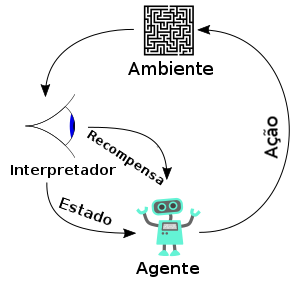
\includegraphics[width=10cm]{imagens/ciclo_rl_agente.png}}
\small{Fonte: Super Data Science}
\label{fig:ciclo_rl}
\end{figure}

O aprendizado por reforço possui dois tipos de configuração, o \textit{offline} e \textit{online} como é chamado na literatura \cite{sutton1998introduction}. Em uma configuração \textit{offline}, a experiência adquirida \textit{a priori} e então é usada para o aprendizado. Isso é um contraste com a configuração \textit{online} onde os dados tornam disponíveis em uma ordem sequencial e são usados para progressivamente atualizar o comportamento do agente.

\subsubsection{Processo de decisão de Markov}

A forma básica de modelar o aprendizado por reforço é seguindo um processo de Markov. O processo de Markov é definido como a probabilidade do estado futuro depender apenas do estado atual \cite{bellman1957markovian}. Sem depender de nenhuma das ações e estados anteriores. Isso quer dizer:
\begin{equation}
P(s_{t+1} \mid {s_0,a_0,s_1,a_1 , ... ,s_t,a_t}) = P( s_{t+1} \mid {s_t,a_t} )
\label{eq:eq1}
\end{equation}

Para um agente que está em um estado e realiza uma certa ação em um ambiente, acontecerá com que o depois dessa ação o agente se encontre em um novo estado em relação ao estado anterior, e então uma determinada recompensa é dada pela ação tomada. A função de recompensa define a meta que o agente do aprendizado por reforço deve atingir. O objetivo desse agente é maximizar a recompensa que ele recebe ao longo do tempo.

Então com a abordagem do agente que utiliza o conceito do processo de Markov, para cada tempo t, são usados os seguintes passos:
\begin{enumerate}
    \item O agente observa o estado atual $s_t$.
    \item O agente faz a ação $a_t$.
    \item O agente recebe a recompensa $r_t = R(s_t, a_t)$.
    \item O agente entra no próximo estado $s_{t+1}$.
\end{enumerate}

Sabendo que na abordagem do processo de Markov é necessário utilizar a equação de Bellman, que especifica qual é a melhor ação que um agente deve tomar em um certo estado \cite{bellman2015applied}. Isto é, a equação de Bellman consegue prever a recompensa gerada de um estado para outro, enquanto, que a função de recompensa só pensa no que é bom em um sentido imediato. A Equação de Bellman é definida como:
\begin{equation}
    V( s_{t} ) =  \underset{a_t}{max}(R(s_t,a_{t}) + \gamma V(s_{t+1}))
    \label{eq:eq2}
\end{equation}

Essa fórmula nos diz qual é o maior valor do estado depois de tomada uma ação.
`$V$' é definido como a “valor” do estado no ambiente.
O valor $\gamma$ (gama) é para admitir um valor de desconto para cada ação tomada. Com a Equação \ref{eq:eq1} e a Equação \ref{eq:eq2} definidas, considerando todas as ações possíveis que um agente pode tomar e a probabilidade de cada ação, é possível ter a equação do processo de decisão de Markov, que é definida como:
\begin{equation}
    V( s_{t} ) = \underset{a_t}{max}( R(s_t,a_{t}) + \gamma \sum_{s_{t+1}} P( s_{t+1} \mid {s_t,a_t} ) V(s_{t+1}) )
\end{equation}

Antes do processo de decisão de Markov, o que acontecia é que todas ações eram tomadas em um ambiente determinístico. Mas com a inserção de incerteza nas ações é possível modelar um ambiente de predição melhor para um lugar mais abstrato e estocástico.